\chapter{Ergebnisse}\label{ch:erg}

In diesem Kapitel werden die Ergebnisse der Experimente dargestellt und ausgewertet.
Die Strukturierung der Experimente werden in \autoref{sec:erg_struk} aufbereitet und in \autoref{sec:erg_time} wird auf die Problematik der Berechnungsdauer eingegangen.
\autoref{sec:erg_LSTM} untersucht Konfigurationen des \ac{LSTM} ohne Verwendung von Extraparametern.
Dabei werden diese speziell nur entweder nach \ac{DR} oder Anzahl der \acp{FP} eingestuft.
In \autoref{sec:erg_LSTM_extra} werden auch Ergebnisse mit Extraparametern hinzugezogen.
% Dabei soll zusätzlich eine beste Konfiguration gefunden werden welche nicht entweder die \ac{DR} oder die \acp{FP} isoliert betrachtet.
Zusätzlich werden in \autoref{sec:erg_vgl} Ergebnisse weiterer Arbeiten mit dieser Arbeit verglichen.

\section{Strukturierung der Experimente}\label{sec:erg_struk}
    Ziel der Experimente ist es, eine Konfiguration zu finden, die bei allen Szenarien des \ac{LID-DS} gut abschneidet.
    Dafür werden wie zuvor beschrieben die N-Gram und Embedding Größe sowie verschiedene Kombinationen der Extraparameter getestet.\par\medskip

    Wieso nicht zusätzlich verschiedene Architekturen, Batchgrößen oder andere Einstellungen in die Konfigurationen einfließen, liegt im Wesentlichen an den vorhandenen Ressourcen.
    Dies wird in \autoref{sec:erg_time} genauer betrachtet.\par\medskip
    Anhand der Experimente wird zunächst untersucht, ob es Konfigurationen des \acp{LSTM} ohne zusätzliche Parameter gibt, welche konkurrenzfähige Ergebnisse liefern können.
    Danach werden auch die zusätzlichen Parameter eingebunden und geprüft wie sie sich auf die Ergebnisse auswirken.
    Um zu untersuchen ergeben sich mehrere Möglichkeiten.
    Eine Möglichkeit besteht darin, dieselben Konfigurationen mit und ohne Extraparametern zu evaluieren und die Ergebnisse zu vergleichen.
    Doch die Hinzunahme von Extraparametern wird die optimale Konfiguration der \acp{LSTM} voraussichtlich verändern, was den Vergleich negativ beeinflusst.
    Eine weitere Möglichkeit könnte es sein, den Mittelwert aller Ergebnisse für jede Extraparameterkonfiguration zu vergleichen.\par\medskip

    Da aber eine beste Konfiguration gesucht wird, ist es möglich, dass viele Konfigurationen, außer der gesuchten, den Mittelwert entscheidend reduzieren.
    Mit dieser Herangehensweise kann es passieren, dass Konfigurationen fälschlicherweise nicht mehr berücksichtigt werden.
    Nichtsdestotrotz wird in \autoref{sec:erg_LSTM_extra} und \autoref{sec:erg_vgl} versucht durch verschiedene Darstellungen einen Vergleich zu ziehen, um so erfolgreiche Konfigurationen darzulegen.

\section{Berechnungsdauer}\label{sec:erg_time}
    Wie erwähnt, ist die Berechnungszeit eine der größten Schwierigkeiten bei der Verwendung dieses \ac{LSTM}-basierten Algorithmus in der \ac{HIDS}.
    Für die Berechnungen wurden zwei verschiedene Grafikkarten auf dem Galaxy Cluster der Universität Leipzig genutzt.
    Das EPS CWE-$434$ sowie das ZipSlip Szenario wurden auf einer NVIDIA Tesla V100 Grafikkarte berechnet und für die restlichen kleineren Szenarien wurde eine NVIDIA RTX 2080 Ti verwendet.
    Die Trainingszeit spielt für den Live-Betrieb eine untergeordnete Rolle, da das Training nur einmalig durchgeführt werden muss.
    Relevanter ist die Berechnungszeit, die für die Auswertung der Testdaten benötigt wird.
    Diese durchschnittlichen Berechnungszeiten werden im Folgenden für die verschiedenen Szenarien gelistet.\par\medskip
    \begin{table}[ht]
        \centering
        \begin{tabular}{lr}
            \hline
            \rowcolor{GruvGray!36}
            \multicolumn{2}{c}{Berechnungszeiten der verschiedenen Szenarien}\\
            \toprule
            Szenario &  $\overline{Detection Time}$ in min\\
            \midrule
            \rowcolor{GruvGray!16}
            CVE-$2017$-$7529$ & $16.22$ \\
            CVE-$2014$-$0160$ & $34.48$ \\
            \rowcolor{GruvGray!16}
            Bruteforce CWE-$307$ & $53.69$ \\
            CVE-$2012$-$2122$ & $55.87$ \\
            \rowcolor{GruvGray!16}
            CVE-$2019$-$5418$ & $155.69$ \\
            CVE-$2018$-$3760$ & $171.56$ \\
            \rowcolor{GruvGray!16}
            PHP CWE-$434$ & $193.55$ \\
            SQL Injection CWE-$89$ & $212.00$ \\
            \rowcolor{GruvGray!16}
            EPS CWE-$434$ & $1157.83$ \\	
            ZipSlip & $2253.75$ \\	
            \hline
        \end{tabular}
        \caption[Ergebnisse Berechnungsdauer Szenarien]{Durchschnittliche Berechnungszeiten zur Bestimmung der Anomaliescores aller Testdaten der einzelnen Szenarien.}
        \label{tab:LSTM_erg_time}
    \end{table}
    Die beiden größten Szenarien benötigen trotz der besseren Grafikkarte wesentlich länger.
    Um die in \autoref{tab:LSTM_erg_time} beschriebenen Ergebnisse zu erzielen, wurden einige Konfigurationen nicht betrachtet.
    So wurde das \ac{OHE} aufgrund der Vektorgröße nicht mit dem W2E verglichen.
    Auch wurden die möglichen Parameter sowie Parametergrößen stark eingeschränkt, um die Anzahl der zu berechnenden Konfigurationen gering zu halten.
    Für die Auswahl wurden Tests auf kleineren Szenarien durchgeführt.
    
    Bei größeren Eingaben, also $n>2$ oder $e>8$ reicht auch der Speicher der NVIDIA Tesla V100 Grafikkarte für das ZipSlip Szenario nicht mehr aus.
    Das mindert die Vergleichbarkeit der Ergebnisse, was die Erkenntnisse dieser Arbeit aber nur geringfügig beeinflusst, dies wird in \autoref{ch:folgerungen} nochmal aufgegriffen.
    Konfigurationen, welche ein Ergebnis für das ZIPSlip Szenario beinhalten, sind blau hervorgehoben.

    \sectionmark{LSTM Ansatz}
    \section{\NoCaseChange{\ac{LSTM}} Ansatz}\label{sec:erg_LSTM}
    \sectionmark{LSTM Ansatz}

    Im ersten Schritt der Auswertung wird die \ac{DR} isoliert betrachtet.
    Dabei werden nur Konfigurationen einbezogen, die keine zusätzlichen Parameter der System Calls enthalten.
    Alle Konfigurationen verwenden dabei \textit{Thread Aware} N-Gramme, also nur System Calls mit derselben ThreadID werden in ein N-Gram aufgenommen.
    In \autoref{tab:LSTM_erg} sind die zehn besten Ergebnisse dargestellt.
    Die durchschnittliche \ac{DR} von $0.71$ bei $14.56$ Fehlern pro Szenario zeigt, dass es generell möglich ist mit \acp{LSTM} eine Anomalieerkennung auf Basis von System Calls umzusetzen.
    Eine klarer Zusammenhang zwischen Embedding Größe ($e$) oder N-Gram Größe ($n$) und der \ac{DR} ist dabei nicht direkt zu erkennen.
    So hat die beste Konfiguration mit einer N-Gram Größe von $10$ und einer Embedding Größe von $4$ also $10 \cdot 4=40$ Eingangsneuronen.
    Hingegen hat die Konfiguration aus Zeile $4$ nur $2 \cdot 4 = 8$ Eingangsneuronen.
    Beide Konfigurationen erzielen dabei sehr ähnliche Ergebnisse mit einer durchschnittlichen \ac{DR} von $0.71$ und $14.56$ \acp{FP} beziehungsweise $0.68$ und $12.89$.
    Dies weist darauf hin, dass mit unterschiedlichen Konfigurationen unterschiedliche Zusammenhänge zwischen den System Call Sequenzen gelernt werden können.

    \begin{table}[ht]
        \centering
        \begin{tabular}{rrrr}
            \hline
            \rowcolor{GruvGray!36}
            \multicolumn{4}{c}{Ohne Extraparameter nach \ac{DR}}\\
            \toprule
            $n$ & $e$ & $\overline{\ac{FP}}$ & $\overline{\ac{DR}}$ \\
            \midrule
            \rowcolor{GruvGray!16}
            $10$ & 	$4$ & 	$14.56$ & 	$0.71$  \\
            $6$ & 	$6$ & 	$22.22$ & 	$0.69$  \\
            \rowcolor{GruvGray!16}
            $2$ & 	$10$ & 	$9.22$  & 	    $0.68$  \\
            $2$ & 	$4$ & 	$12.89$ & 	$0.68$  \\
            \rowcolor{GruvGray!16}
            $10$ & 	$8$ & 	$17.78$ & 	$0.67$  \\
            \rowcolor{CTblue!16}
            $2$ & 	$6$ & 	$20.60$ & 	$0.64$  \\
            \rowcolor{GruvGray!16}
            $6$ & 	$4$ & 	$11.34$ & 	$0.58$  \\
            $10$ & 	$10$ & 	$5.78$ & 	    $0.56$  \\
            \rowcolor{GruvGray!16}
            $10$ & 	$6$ & 	$6.44$ & 	    $0.56$  \\
            $6$ & 	$10$ & 	$7.33$ & 	    $0.56$  \\
            \hline
        \end{tabular}
        \caption[Ergebnisse \ac{DR} ohne Extraparameter]{Konfigurationen mit den $10$ höchsten \acp{DR}. 
                 Dabei wurden nur Konfigurationen betrachtet die keine Extraparameter nutzen.
                 Alle N-Gramme sind \textit{Thread Aware}.
                 Blaue Zeilen enthalten Ergebnisse des ZipSlip Szenarios.}
        \label{tab:LSTM_erg}
    \end{table}
    \newpage
    Im zweiten Schritt der Auswertung werden die besten Ergebnisse nur im Bezug auf die Anzahl der Fehlalarme, also \acp{FP} untersucht.
    In \autoref{tab:LSTM_erg_FP} werden wieder \textit{Thread Aware} N-Gramme genutzt und nur Ergebnisse mit $\ac{DR}>0.5$ einbezogen.

    \begin{table}[ht]
        \centering
        \begin{tabular}{rrrr}
            \hline
            \rowcolor{GruvGray!36}
            \multicolumn{4}{c}{Ohne Extraparameter, nach \ac{FP}}\\
            \toprule
            $n$ & $e$ & $\overline{\ac{FP}}$ & $\overline{\ac{DR}}$ \\
            \midrule
            \rowcolor{GruvGray!16}
            $10$ & 	$10$ & 	$5.78$ & 	    $0.56$ \\
            $10$ & 	$6$ & 	$6.44$ & 	    $0.56$ \\
            \rowcolor{GruvGray!16}
            $6$ & 	$10$ & 	$7.33$ & 	    $0.56$ \\
            \rowcolor{CTblue!16}
            $2$ & 	$8$ & 	$8.40$ & 	    $0.50$ \\
            \rowcolor{GruvGray!16}
            $2$ & 	$10$ & 	$9.22$ & 	    $0.68$ \\
            $6$ & 	$4$ & 	$11.34$ & 	$0.58$ \\
            \rowcolor{GruvGray!16}
            $2$ & 	$4$ & 	$12.89$ & 	$0.68$ \\
            $10$ & 	$4$ & 	$14.56$ & 	$0.71$ \\
            \rowcolor{GruvGray!16}
            $10$ & 	$8$ & 	$17.78$ & 	$0.67$ \\
            \rowcolor{CTblue!16}
            $2$ & 	$6$ & 	$20.60$ & 	$0.64$ \\
            \hline
        \end{tabular}
        \caption[Ergebnisse \ac{FP}-Rate ohne Extraparameter]{Konfigurationen mit den $10$ niedrigsten \acp{FP}. 
                 Es werden nur Konfigurationen betrachtet die keine Extraparameter nutzen.
                 Alle N-Gramme sind \textit{Thread Aware}.
                 Es wurden nur Konfigurationen mit $\ac{DR}>0.5$ einbezogen.
                 Nur blaue Zeilen enthalten Ergebnisse des ZipSlip Szenarios.}
        \label{tab:LSTM_erg_FP}
    \end{table}
    
    Hierbei überschneiden sich viele Konfigurationen aus \autoref{tab:LSTM_erg}.
    Das liegt vor allem daran, dass es nur wenig mehr als zehn Konfigurationen ohne Extraparameter mit einer $\ac{DR}>0.5$ gibt.
    Wieder lässt sich kein klarer Trend in den Konfigurationen von N-Gram und Embedding Größe erkennen.\par\medskip

    Doch die Tabelle kann genutzt werden, um noch einmal auf die Schwierigkeit der Auswahl der besten Konfigurationen hinzuweisen.
    Ist eine Konfiguration mit hoher \ac{DR} oder eine Konfiguration mit wenigen \acp{FP} zu bevorzugen?
    Oder konkret wie in diesem Fall, ist eine $\ac{DR}=0.71$ bei im Schnitt ca. $15$ Fehlern in grob acht Stunden Testaufnahmen der Konfiguration mit einer $\ac{DR}=0.56$ bei ca. $6$ Fehlern zu bevorzugen?
    Der Versuch eine beste Konfiguration auszuwählen werden nach Betrachtung der Konfigurationen mit Extraparametern unternommen.\par\medskip

    In \autoref{tab:LSTM_pro_szenario} werden für die beiden besten Konfigurationen alle Szenarien aufgeschlüsselt.
    Zu erkennen ist , dass in dem $CVE-2014-0160$ wie auch dem $CVE-2012-2122$ Szenario bei der Konfiguration mit der besten \ac{DR} insgesamt keine Angriffe erkannt werden. 
    Interessanterweise löst die Konfiguration mit der geringsten \ac{FP}-Rate das $CVE-2014-0160$ Szenario mit nur einem Fehler.
    Ein Szenario, in welchem das \ac{LSTM} typischerweise schlecht abschneidet.\par\medskip
    \begin{table}[ht]
        \centering
        \begin{tabular}{lrrcrr}
            \hline
            \rowcolor{GruvGray!36}
            \multicolumn{6}{c}{Ohne Extraparameter - pro Szenario}\\
            \toprule
            Szenario & $\overline{\ac{FP}}$ & $\overline{\ac{DR}}$ & vs & $\overline{\ac{FP}}$ & $\overline{\ac{DR}}$ \\
            \midrule
            \rowcolor{GruvGray!16}
            $Bruteforce\_CWE-307$   &$60$ &$0.94$ & x & $15$ & 	$1.00$ \\
            $CVE-2012-2122$        &$8$  &$0.01$ & x & $4$ & 	$0.03$ \\
            \rowcolor{GruvGray!16}
            $CVE-2014-0160$        &$3$  &$0.00$ & x & $1$ & 	$0.99$ \\
            $CVE-2017-7529$        &$1$  &$0.99$ & x & $0$ & 	$0.05$ \\
            \rowcolor{GruvGray!16}
            $CVE-2018-3760$        &$11$ &$1.00$ & x & $9$ & 	$0.01$ \\
            $CVE-2019-5418$        &$32$ &$1.00$ & x & $12$ & 	$1.00$ \\
            \rowcolor{GruvGray!16}
            $EPS\_CWE-434$          &$14$ &$1.00$ & x & $9$ & 	$1.00$ \\
            $PHP\_CWE-434$          &$4$  &$0.96$ & x & $1$ & 	$1.00$ \\
            \rowcolor{GruvGray!16}
            $SQL\_Injection\_CWE-89$ &$1$  &$0.46$ & x & $1$ & 	$0.00$ \\
            $ZipSlip$                & x & x & x & x & x \\
            \hline
        \end{tabular}
        \caption[Ergebnisse bester Konfigurationen auf Szenarien aufgeschlüsselt]{Auflistung der einzelnen Szenarien für die Konfiguration mit der höchsten \ac{DR} ($n=10$, $e=4$) links und der wenigsten \acp{FP} ($n=10$, $e=10$)}
        \label{tab:LSTM_pro_szenario}
    \end{table}
    Dies zeigt sich auch in \autoref{tab:LSTM_pro_szenario_allg}. 
    Hier wird die durchschnittliche \ac{DR} für alle Szenarien dargestellt.
    In vier Szenarien werden im Schnitt nur sehr wenige Angriffe erkannt.
    Dazu gehören das $ZipSlip$ Szenario sowie $CVE-2012-2122$, $CVE-2014-0160$ und das $Bruteforce\_CWE-307$.
    Problematisch sind dabei speziell das $ZipSlip$ Szenario sowie das $Bruteforce\_CWE-307$ Szenario, da sie zusätzlich zu einer geringen \ac{DR} auch zu vielen \acp{FP} führen.
    \begin{table}[H]
        \centering
        \small
        \begin{tabular}{lrr}
            \hline
            \rowcolor{GruvGray!36}
            \multicolumn{3}{c}{Ohne Extraparameter - pro Szenario}\\
            \toprule
            Szenario & $\overline{\ac{FP}}$ & $\overline{\ac{DR}}$ \\
            \midrule
            \rowcolor{GruvGray!16}
            $Bruteforce\_CWE-307$  &$22.09$ & 	$0.29$ \\
            $CVE-2012-2122$        &$14.00$ & 	$0.02$ \\
            \rowcolor{GruvGray!16}
            $CVE-2014-0160$        &$3.25$ & 	$0.08$ \\
            $CVE-2017-7529$       &$0.58$  & 	$0.82$ \\
            \rowcolor{GruvGray!16}
            $CVE-2018-3760$        &$17.00$ & 	$1.00$ \\
            $CVE-2019-5418$       &$12.17$  & 	$0.58$ \\
            \rowcolor{GruvGray!16}
            $EPS\_CWE-434$         &$14.80$ & 	$1.00$ \\
            $PHP\_CWE-434$         &$10.09$ & 	$0.91$ \\
            \rowcolor{GruvGray!16}
            $SQL\_Injection\_CWE-89$&$9.81$ & 	$0.95$ \\
            $ZipSlip$              &$35.5$ & $0.15$ \\
            \hline
        \end{tabular}
        \caption[Durschnittliche Ergebnisse auf Szenarien aufgeschlüsselt]{Durchschnittliche \ac{DR} und \acp{FP} für alle Szenarien mit Konfigurationen ohne Extraparametern.}
        \label{tab:LSTM_pro_szenario_allg}
    \end{table}


\section{Einsatz von Extraparameter}\label{sec:erg_LSTM_extra}
    \begin{table}[ht]
        \centering
        \begin{tabular}{rrrrrrr}
            \hline
            \rowcolor{GruvGray!36}
            \multicolumn{7}{c}{Mit Extraparametern nach \ac{DR}}\\
            \toprule
            $n$ & $e$ & \textit{rv} & \ac{TCF} & \textit{time} & $\overline{\ac{FP}}$ & $\overline{\ac{DR}}$ \\
            \midrule
            \rowcolor{GruvGray!16}
            $6$ & 	$8$ & 	$1$ & 	$1$ & 	$1$ & 	$22.89$ & 	$0.88$ \\
            $10$ & 	$4$ & 	$1$ & 	$1$ & 	$0$ & 	$14.00$ & 	$0.76$ \\
            \rowcolor{GruvGray!16}
            $10$ & 	$8$ & 	$0$ & 	$1$ & 	$1$ & 	$18.56$ & 	$0.76$ \\
            $10$ & 	$4$ & 	$0$ & 	$1$ & 	$0$ & 	$5.00$ & 	    $0.74$ \\
            \rowcolor{GruvGray!16}
            $10$ & 	$4$ & 	$1$ & 	$0$ & 	$0$ & 	$13.78$ & 	$0.74$ \\
            $10$ & 	$4$ & 	$1$ & 	$1$ & 	$1$ & 	$22.33$ & 	$0.74$ \\
            \rowcolor{GruvGray!16}
            $10$ & 	$4$ & 	$0$ & 	$0$ & 	$0$ & 	$14.56$ & 	$0.71$ \\
            $6$ & 	$8$ & 	$1$ & 	$1$ & 	$0$ & 	$9.00$ & 	    $0.70$ \\
            \rowcolor{GruvGray!16}
            \rowcolor{CTblue!16}
            $2$ & 	$8$ & 	$1$ & 	$1$ & 	$1$ & 	$14.00$ & 	$0.70$ \\
            $6$ & 	$4$ & 	$1$ & 	$0$ & 	$1$ & 	$18.22$ & 	$0.70$ \\
            \hline
        \end{tabular}
        \caption[Ergebnisse nach \ac{DR} mit Extraparametern]{Konfigurationen mit den $10$ höchsten \acp{DR}. 
                 Es wurden Konfigurationen mit und ohne Extraparameter betrachtet.
                 Alle N-Gramme sind \textit{Thread Aware}.
                 Nur blaue Zeilen enthalten Ergebnisse des ZipSlip Szenarios.}
        \label{tab:LSTM_par_erg}
    \end{table}
    In \autoref{tab:LSTM_par_erg} finden sich die Ergebnisse der Konfigurationen mit und ohne Extraparametern. 
    Wieder werden die Ergebnisse zunächst nach der besten \ac{DR} eingestuft.
    Als erstes fällt dabei ins Auge, dass die besten sechs Konfigurationen Extraparameter verwenden.
    % Dies gibt einen Hinweis darauf, dass die Parameter im Einsatz in Kombination mit einem \ac{LSTM} sehr nützlich sind.
    Im Vergleich der besten Konfigurationen werden ohne Extraparameter wie oben beschrieben eine \ac{DR} von $0.71$ bei durchschnittlich $14.56$ Fehlern erreicht.
    Mit Extraparametern beträgt die höchste \ac{DR} $0.88$ bei durchschnittlich $22.89$ Fehlern.
    Also auf die \ac{DR} bezogen eine deutliche Verbesserung.\par\medskip

    Im Gegensatz zu \autoref{tab:LSTM_erg} ist diesmal ein Zusammenhang zwischen der Embedding sowie N-Gram-Größe und der Ergebnisqualität zu erkennen.
    So liefert die Konfiguration mit $n=10$ und $e=4$ für viele Extraparameterkombinationen gute Ergebnisse.
    Sie kommt fünf mal unter den besten $7$ Ergebnissen vor.
    Zusätzlich ist sie auch die beste Konfiguration ohne Extraparameter.
    Es ist auch die einzige Konfiguration ohne Extraparametern, die es in unter die besten zehn geschafft hat.
    Das beste Ergebnis hinsichtlich der \ac{DR} liefert allerdings eine N-Gram Größe von $6$ bei einer Embedding Größe von $8$.\par\medskip
    %In den sechs besten Ergebnissen nach der \ac{DR} wird die \ac{TCF} eingesetzt.

    Auch bei den Ergebnissen nach den geringsten \acp{FP} in \autoref{tab:LSTM_FP} verwenden sieben der besten zehn Konfigurationen Extraparameter, darunter auch die besten drei.
    So kann mit nur durchschnittlich $4.66$ Fehlalarmen bei einer \ac{DR} von $0.67$ eine deutliche Steigerung gegenüber durchschnittlich $5.78$ Fehlern bei einer \ac{DR} von $0.56$  erreicht werden.
    Auch hier kommen die Konfiguration $n=10$ und $e=4$ unter den besten Ergebnissen vor.
    Die beiden besten Ergebnisse\marginpar{nach \ac{DR} und \ac{FP}} erzielt die Konfiguration $n=6$ und $e=8$.

    \begin{table}[ht]
        \centering
        \begin{tabular}{rrrrrlr}
            \hline
            \rowcolor{GruvGray!36}
            \multicolumn{7}{c}{Mit Extraparametern nach \ac{FP}}\\
            \toprule
            $n$ & $e$ & \textit{rv} & \ac{TCF} & \textit{time} & $\overline{\ac{FP}}$ & $\overline{\ac{DR}}$ \\
            \midrule
            \rowcolor{GruvGray!16}
            $6$ & 	$8$ & 	$0$ & 	$0$ & 	$1$ & 	$4.66$ & 	 	$0.67$ \\
            $10$ & 	$4$ & 	$0$ & 	$1$ & 	$0$ & 	$5$    & 	$0.74$\\
            \rowcolor{GruvGray!16}
            $10$ & 	$6$ & 	$0$ & 	$1$ & 	$0$ & 	$5.66$ & 	 	$0.60$ \\
            $10$ & 	$10$ & 	$0$ & 	$0$ & 	$0$ & 	$5.78$ & 	 	$0.56$ \\
            \rowcolor{GruvGray!16}
            $6$ & 	$4$ & 	$0$ & 	$0$ & 	$1$ & 	$5.80$ & 	 	$0.64$ \\
            $6$ & 	$6$ & 	$1$ & 	$1$ & 	$1$ & 	$6.33$ & 	 	$0.66$ \\
            \rowcolor{GruvGray!16}
            $10$ & 	$6$ & 	$1$ & 	$0$ & 	$0$ & 	$6.33$ & 	 	$0.55$ \\
            $10$ & 	$6$ & 	$0$ & 	$0$ & 	$0$ & 	$6.44$ & 	 	$0.56$ \\
            \rowcolor{GruvGray!16}
            $6$ & 	$10$ & 	$0$ & 	$0$ & 	$0$ & 	$7.33$ & 	 	$0.56$ \\
            $6$ & 	$6$ & 	$0$ &  	$0$ &  	$1$ &  	$7.89$ &   		$0.64$ \\ 
            \hline
        \end{tabular}
        \caption[Ergebnisse nach \ac{FP} mit Extraparametern]{Konfigurationen mit den $10$ niedrigsten \ac{FP}-Raten. 
                 Es wurden Konfigurationen mit und ohne Extraparameter betrachtet.  Alle N-Gramme sind \textit{Thread Aware}.
                 Auch hier kommen bei den meisten Konfigurationen die Extraparameter zum Einsatz.}
        \label{tab:LSTM_FP}
    \end{table}

    Wie in \autoref{sec:erg_struk} beschrieben kann die Betrachtung des Mittelwertes auch für nicht repräsentative Ergebnisse sorgen.
    Dadurch können gute Konfigurationen übersehen werden.
    In \autoref{tab:LSTM_pro_szenario_allg_param} ist keine deutliche Verbesserung der Ergebnisse mit Hinzunahme der Extraparameter zu erkennen.
    Dies kann zu einem frühzeitigen Ausschluss bestimmter Konfigurationen führen.
    Die Verbesserungen zu \autoref{tab:LSTM_pro_szenario_allg} werden mit blau und die Verschlechterungen mit rot dargestellt.
    Diese Ergebnisse werden für jedes Szenario in \autoref{fig:erg_vgl_extra} visualisiert.
    In Blau werden die Ergebnisse mit Verwendung der Extraparameter dargestellt und in Rot ohne Extraparameter.
    Die Höhe der Kreise gibt die \ac{DR} an und die Größe die Anzahl der \acp{FP}.
    Eine Abweichung der Mittelwerte ist in Szenario $CVE-2014-0160$ sowie in Szenario $CVE-2017-7529$ zu erkennen.
    Werden die besten Konfigurationen betrachtet, stellt sich ein anderes Bild dar.
    \par\medskip

    \begin{table}[ht]
        \centering
        \begin{tabular}{lrrrr}
            \hline
            \rowcolor{GruvGray!36}
            \multicolumn{5}{c}{Mit Extraparameter - pro Szenario}\\
            \toprule
            Szenario & $\overline{\ac{FP}}$ & $\Delta$ & $\overline{\ac{DR}}$ & $\Delta$ \\
            \midrule
            \rowcolor{GruvGray!16}
            $Bruteforce\_CWE-307$  &$25.82$ &{\color{CTred} $3.73$} & 	$0.30$  &{\color{CTred}$0.01$}\\ 
            $CVE-2012-2122$        &$11.82$ &{\color{CTblue}$2.19$} & 	$0.03$  &{\color{CTblue}$0.01$}\\
            \rowcolor{GruvGray!16}
            $CVE-2014-0160$        &$5.95$ &{\color{CTred}$2.70$}  & 	$0.01$  &{\color{CTred}$0.07$}\\
            $CVE-2017-7529$        &$1.25$  &{\color{CTblue}$0.67$} & 	$0.90$  &{\color{CTblue}$0.08$}\\
            \rowcolor{GruvGray!16}
            $CVE-2018-3760$        &$8.82$ &{\color{CTblue}$8.18$}  &	$1.00$  &{\color{CTblue}$0.00$}\\
            $CVE-2019-5418$       &$7.00$  &{\color{CTblue}$5.17$}  &	$0.58$  &{\color{CTblue}$0.00$}\\
            \rowcolor{GruvGray!16}
            $EPS\_CWE-434$         &$18.56$ &{\color{CTred}$3.76$} & 	$0.97$  &{\color{CTred}$0.03$}\\
            $PHP\_CWE-434$         &$13.22$ &{\color{CTred}$3.13$} & 	$0.91$  &{\color{CTblue}$0.00$}\\
            \rowcolor{GruvGray!16}
            $SQL\_Injection\_CWE-89$&$25.51$ &{\color{CTred}$15.70$}& 	$0.99$  &{\color{CTblue}$0.04$}\\
            \rowcolor{CTred!16}
            $ZipSlip$              &$11.64$ &{\color{CTblue}$23.86$} &   $0.19$ &{\color{CTblue}$0.04$}\\
            \hline
        \end{tabular}
        \caption[Ergebnisse auf Szenarien aufgeschlüsselt]{Durchschnittliche \ac{DR} und \acp{FP} für alle Szenarien mit Konfigurationen ohne Extraparametern.
        In den Mittelwert des ZipSlip-Szenarios fließen weniger Werte ein.}
        \label{tab:LSTM_pro_szenario_allg_param}
    \end{table}

    \begin{figure}[H]
        \centering
        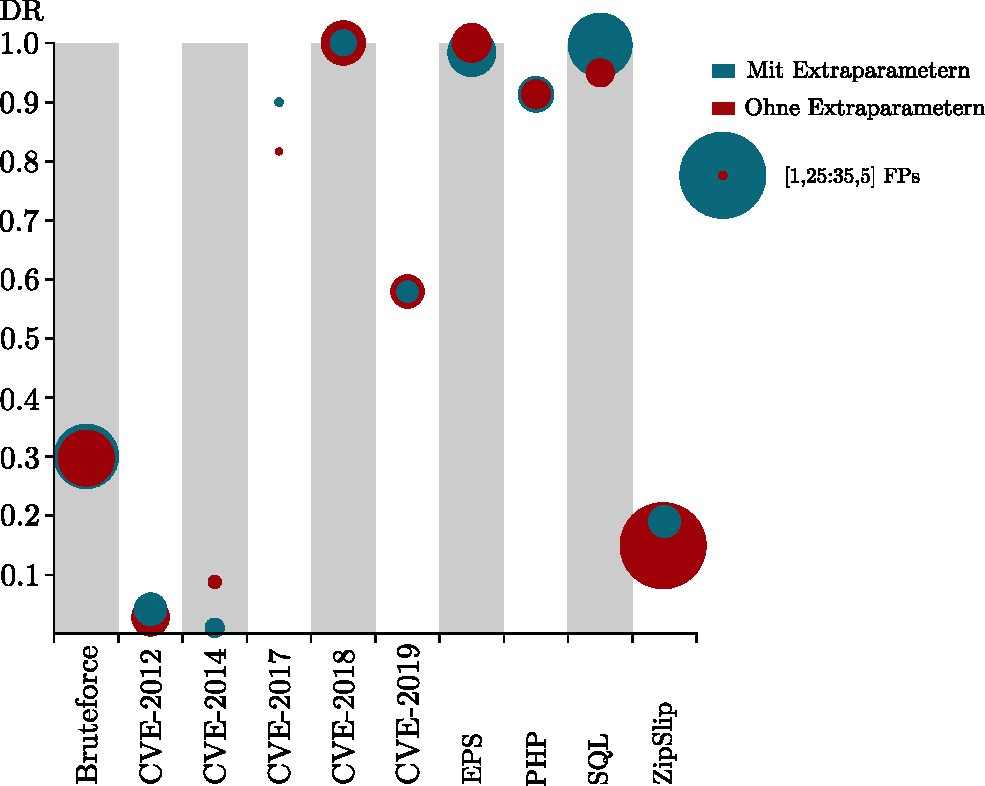
\includegraphics[width=1\textwidth]{images/Erg_balls.pdf}
        \caption[Mittelwerte pro Szenario mit/ohne Extraparametern]{Mittelwerte der \ac{DR} und \acp{FP} pro Szenario für Konfigurationen ohne Extraparametern (rot) und mit Extraparametern (blau).
                                                                    Anzahl der \acp{FP} gibt Größe der Kreise wieder.}\label{fig:erg_vgl_extra}
    \end{figure}

    \newpage
    In  \autoref{tab:LSTM_vs_alternative} und \autoref{tab:LSTM_vs} werden die zwei Gewinnerkonfigurationen mit Extraparametern mit jeweils den Gewinnerkonfigurationen ohne Extraparametern gegenübergestellt.
    Dabei werden die Ergebnisse jedes Szenarios angegeben. 
    Im Gegensatz zu den Mittelwerten zuvor ist eine klare Verbesserung zu erkennen.
    Dies spiegelt sich auch in der Visualisierung der beiden Tabellen in \autoref{fig:erg_vgl_dr} und \autoref{fig:erg_vgl_fp} wieder.
    Auffällig dabei ist die unterschiedliche Verteilung welche Szenarien vergleichsweise gut gelöst werden.
    Ohne Extraparameter wird das $CVE-2014-0160$ Szenario mit einer hohen \ac{DR} und geringer \acp{FP} gelöst.
    Diese ist wie in \autoref{tab:LSTM_pro_szenario_allg} beschrieben im Schnitt eines der am schlechtesten gelösten Szenarien.
    Hingegen werden die vermeintlich einfachen Szenarien wie das $CVE-2018-5418$ nicht gut gelöst.
    Im Vergleich werden mit Extraparametern das Bruteforce, $CVE-2012-2122$ und das $CVE-2014-0160$ Szenario bezüglich \ac{DR} schlecht gelöst und alle anderen haben eine sehr hohe \ac{DR} bei einer geringen Anzahl an Fehlalarmen.

    \begin{table}[H]
        \centering
        \begin{tabular}{lrrrrr}
            \hline
            \rowcolor{GruvGray!36}
            \multicolumn{6}{c}{Vergleich beste Konfiguration nach \ac{DR}}\\
            \hline
            Szenario & \ac{FP} & \ac{DR} & vs.\ & \acp{FP} & \ac{DR}\\
            \toprule
            \rowcolor{GruvGray!16}
            Bruteforce CWE-307    & $60$ & $0.94$ & x & {\color{CTblue}$29$} &{\color{CTblue}$0.94$} \\
            CVE-2012-2122 	      & $8$ & $0.01$ & x & {\color{CTred}$18$} &{\color{CTblue}$0.99$} \\
            \rowcolor{GruvGray!16}
            CVE-2014-0160 	      & $3$ & $0.00$ & x & {\color{CTred}$13$} &{\color{CTblue}$0.03$} \\
            CVE-2017-7529 	      & $1$  & $0.99$ & x & {\color{CTblue}$0$} &{\color{CTblue}$0.99$} \\
            \rowcolor{GruvGray!16} 
            CVE-2018-3760 	      & $11$  & $1.00$ & x & {\color{CTblue}$4$} &{\color{CTblue}$1.00$} \\
            CVE-2019-5418 	      & $32$  & $1.00$ & x & {\color{CTblue}$7$} &{\color{CTblue}$1.00$} \\
            \rowcolor{GruvGray!16}
            EPS CWE-434 	      & $14$ & $1.00$ & x & {\color{CTred}$29$} &{\color{CTblue}$1.00$} \\
            PHP CWE-434 	      & $4$ & $0.96$ & x & {\color{CTred}$24$} &{\color{CTblue}$.1.00$} \\
            \rowcolor{GruvGray!16}
            SQL Injection CWE-89 &	$1$ & $0.46$ & x & {\color{CTred}$82$} &{\color{CTblue}$1.00$} \\
            ZIP Slip              & xxx  & xxx        & x & xxx  & xxx \\
            \hline
        \end{tabular}
        \caption[Vergleich \ac{DR} ohne Extraparameter vs.\ mit Extraparameter ]{Vergleich bester Ergebnisse. Höchste \ac{DR} links mit folgenden Parametern: $n=6, e=8, rv=0, \ac{TCF}=0, time=0$.
                Höchste \ac{DR} rechts mit folgenden Parametern: $n=6, e=8, rv=1, \ac{TCF}=1, time=1$.
                Eine Verschlechterung wird mit Rot hervorgehoben, ansonsten Blau.}
        \label{tab:LSTM_vs_alternative}
    \end{table}

    \begin{table}[H]
        \centering
        \begin{tabular}{lrrrrr}
            \hline
            \rowcolor{GruvGray!36}
            \multicolumn{6}{c}{Vergleich beste Konfiguration nach \ac{FP}}\\
            \hline
            Szenario & \ac{FP} & \ac{DR} & vs & \acp{FP} & \ac{DR}\\
            \toprule
            \rowcolor{GruvGray!16}
            Bruteforce CWE-307    & $15$ & $1.00$ & x & {\color{CTblue}$10$} &{\color{CTred}$0.07$} \\
            CVE-2012-2122 	      & $4$ & $0.03$& x & {\color{CTred}$10$} &{\color{CTblue}$0.02$} \\
            \rowcolor{GruvGray!16}
            CVE-2014-0160 	      & $1$ & $0.99$ & x & {\color{CTred}$5$} &{\color{CTred}$0.00$} \\
            CVE-2017-7529 	      & $0$  & $0.05$ & x & {\color{CTred}$3$} &{\color{CTblue}$0.99$} \\
            \rowcolor{GruvGray!16} 
            CVE-2018-3760 	      & $9$  & $0.01$ & x & {\color{CTblue}$0$} &{\color{CTblue}$1.00$} \\
            CVE-2019-5418 	      & $12$  & $1.00$ & x & {\color{CTblue}$3$} &{\color{CTred}$0.99$} \\
            \rowcolor{GruvGray!16}
            EPS CWE-434 	      & $9$ & $1.00$ & x & {\color{CTblue}$9$} &{\color{CTblue}$1.00$} \\
            PHP CWE-434 	      & $1$ & $0.00$ & x & {\color{CTblue}$1$} &{\color{CTblue}$1.00$} \\
            \rowcolor{GruvGray!16}
            SQL Injection CWE-89 &	$1$ & $1.00$ & x & {\color{CTblue}$1$} &{\color{CTblue}$1.00$} \\
            ZIP Slip              & xxx  & xxx        & x & xxx  & xxx \\
            \hline
        \end{tabular}
        \caption[Vergleich \ac{FP} ohne Extraparameter vs.\ mit Extraparameter ]{Vergleich bester Ergebnisse.
                Niedrigste \acp{FP} links mit folgenden Parametern: $n=10, e=10, rv=0, \ac{TCF}=0, time=0$.
                Niedrigste \acp{FP} rechts mit folgenden Parametern: $n=6, e=8, rv=0, \ac{TCF}=0, time=1$.
                Eine Verschlechterung wird mit Rot hervorgehoben, ansonsten Blau.}
        \label{tab:LSTM_vs}
    \end{table}
    \begin{figure}[ht]
        \centering
        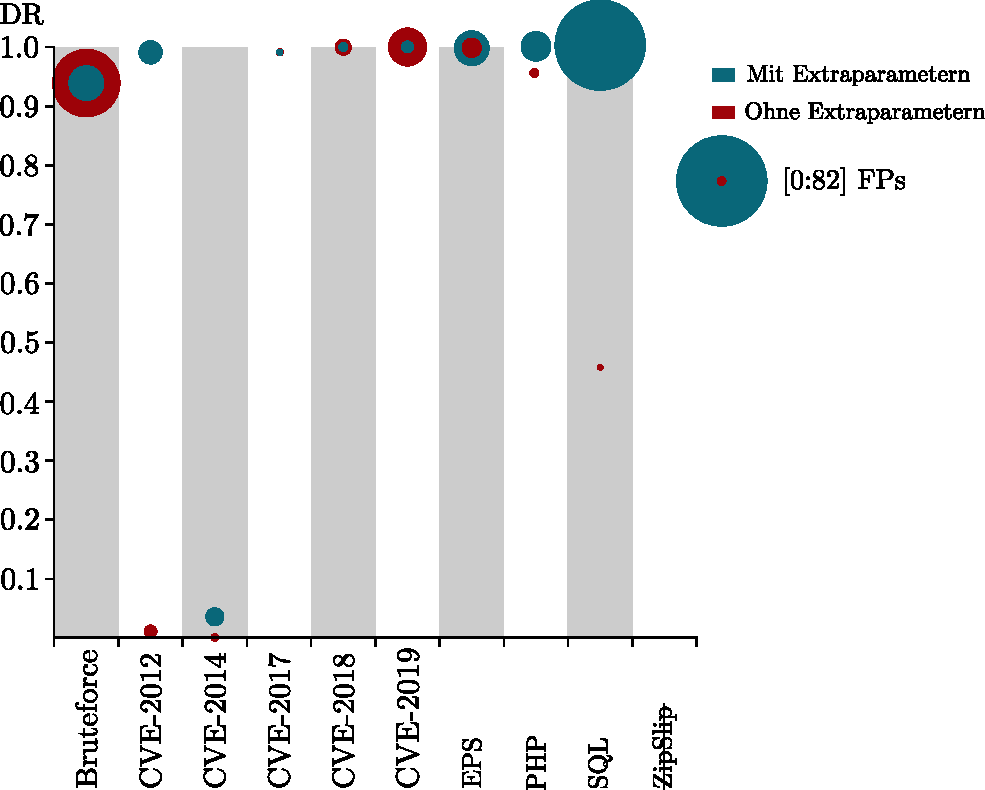
\includegraphics[width=1\textwidth]{images/Erg_balls_fp.pdf}
        \caption[Vergleich \ac{DR} ohne Extraparameter vs.\ mit Extraparameter]{Vergleich bester Ergebnisse bezüglich \ac{DR}. 
            Rot ohne Extraparametern: $n=6, e=8, rv=0, \ac{TCF}=0, time=0$.
            Blau mit Extraparametern: $n=6, e=8, rv=1, \ac{TCF}=1, time=1$.
        }\label{fig:erg_vgl_dr}
    \end{figure}
    \begin{figure}[ht]
        \centering
        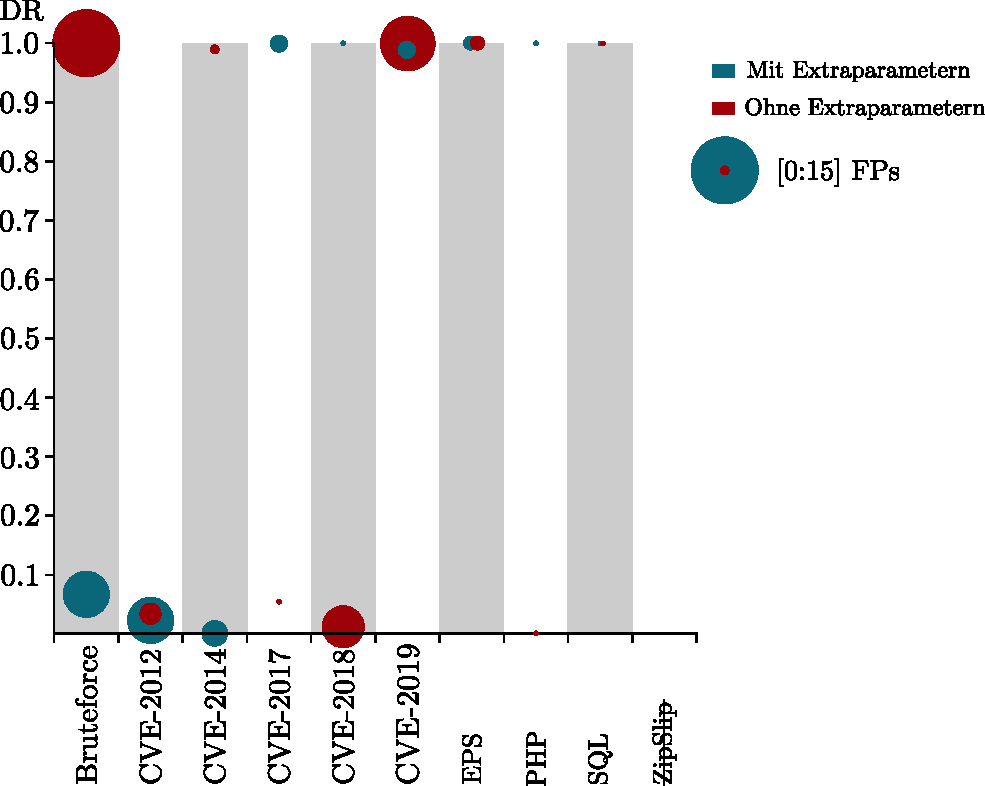
\includegraphics[width=1\textwidth]{images/Erg_balls_dr.pdf}
        \caption[Vergleich \ac{FP} ohne Extraparameter vs.\ mit Extraparameter]{Vergleich bester Ergebnisse bezüglich \acp{FP} mit (blau) und ohne (rot) Extraparameter.
            Rot ohne Extraparametern: $n=10, e=10, rv=0, \ac{TCF}=0, time=0$.
            Blau mit Extraparametern: $n=6, e=8, rv=0, \ac{TCF}=0, time=1$.
        }\label{fig:erg_vgl_fp}
    \end{figure}
\iffalse
    In \autoref{tab:LSTM_para_vgl} wird jeweils der Mittelwert der besten fünf Konfigurationen, ausgewählt nach der besten \ac{DR}, für die verschiedenen Kombinationen der Extraparametern.
    Einmal aufgestellt nach der höchsten \ac{DR} und einmal nach der niedrigsten \ac{FP}-Rate.
    Zu erkennen ist, dass in beiden Fällen Konfigurationen mit Extraparametern mindestens die ersten beiden Plätze belegen.

    \begin{table}[ht]
        \parbox{.45\linewidth}{\centering
            \begin{tabular}{lrrrl}
                \hline
                \rowcolor{GruvGray!36}
                \multicolumn{5}{c}{Sortiert nach $\overline{\ac{DR}}$}\\
                \hline
                td  & \ac{TCF} & rv & $\overline{\ac{FP}}$ & $\overline{\ac{DR}}$ \\
                \toprule
                \rowcolor{GruvGray!16}
                $1$ & $1$ & $1$ & $16.5$ & $0.736$ \\
                $0$ & $1$ & $1$ & $11.8$ & $0.688$ \\
                \rowcolor{GruvGray!16}
                $0$ & $0$ & $0$ & $15.5$ & $0.686$ \\
                $1$ & $0$ & $1$ & $15.6$ & $0.680$ \\
                \rowcolor{GruvGray!16}
                $0$ & $1$ & $0$ & $13.8$ & $0.664$ \\
                $0$ & $0$ & $1$ & $6.7$ & $0.652$ \\
                \rowcolor{GruvGray!16}
                $1$ & $0$ & $0$ & $9.2$ & $0.650$ \\
                $1$ & $1$ & $0$ & $13.5$ & $0.636$ \\
                \hline
            \end{tabular}}
        \hfill
        \parbox{.45\linewidth}{\centering
            \begin{tabular}{lrrrl}
                \hline
                \rowcolor{GruvGray!36}
                \multicolumn{5}{c}{Sortiert nach $\overline{\ac{FP}}$}\\
                \hline
                td  & \ac{TCF} & rv & $\overline{\ac{FP}}$ & $\overline{\ac{DR}}$ \\
                \toprule
                \rowcolor{GruvGray!16}
                $0$ & $0$ & $1$ & $6.7$ & $0.652$ \\
                $1$ & $0$ & $0$ & $9.2$ & $0.650$ \\
                \rowcolor{GruvGray!16}
                $0$ & $1$ & $1$ & $11.8$ & $0.688$ \\
                $1$ & $1$ & $0$ & $13.5$ & $0.636$ \\
                \rowcolor{GruvGray!16}
                $0$ & $1$ & $0$ & $13.8$ & $0.664$ \\
                $0$ & $0$ & $0$ & $15.5$ & $0.686$ \\
                \rowcolor{GruvGray!16}
                $1$ & $0$ & $1$ & $15.6$ & $0.680$ \\
                $1$ & $1$ & $1$ & $16.5$ & $0.736$ \\
                \hline
            \end{tabular}}
        \caption[Parameter Vergleich]{Vergleich Parameter, Auswahl jeweils Mittelwert der besten fünf Ergebnisse nach \ac{DR}. Einmal nach \ac{DR} sortiert links und nach \ac{FP} sortiert rechts}
        \label{tab:LSTM_para_vgl}
    \end{table}

    \fi


\section{Vergleich anderer Arbeiten}\label{sec:erg_vgl}
    Um die Ergebnisse einordnen zu können, wird im Folgenden ein Vergleich zu Arbeiten gezogen, die ebenfalls den \ac{LID-DS} verwenden.
    Dafür steht der \ac{STIDE} von Grimmer et al.~\cite{IDSTHREADGRIMMER2021} zur Verfügung.
    Der Vergleich der beiden besten \ac{LSTM} Konfigurationen und dem \ac{STIDE} Algorithmus wird in \autoref{tab:LSTM_stide_erg} dargestellt.
    Dabei wird im \ac{STIDE} ein \ac{SW} verwendet.
    %Ein \ac{SW} wird ähnlich zu einem n-gram aufgebaut.
    %Dafür werden aber nur die Anomaliescores der einzelnen N-Gramme genommen und gemittelt.
    Ein Anomaliescore mit \ac{SW} beinhaltet in diesem speziellen Fall den Mittelwert von $1000$ Anomaliewerten der N-Gramme. 
    Die \ac{DR} des \ac{STIDE} von $0.986$ wird nicht erreicht, allerdings werden die \acp{FP} um ca. $60\%$ von durchschnittlich $61.5$ auf $22.89$ reduziert.
    
    \begin{table}[ht]
        \centering
        \begin{tabular}{lrrrrrrrr}
            \hline
            \rowcolor{GruvGray!36}
            \multicolumn{9}{c}{Ergebnisse für \ac{LSTM} mit Extraparameter}\\
            \toprule
            Algorithmus & $n$ & $e$ & \ac{SW} & \textit{rv} & \ac{TCF} & \textit{time} & $\overline{\ac{FP}}$ & $\overline{\ac{DR}}$ \\
            \midrule
            \ac{STIDE} & $5$ & int & $1000$ & $0$ & $0$ & $0$ & $61.50$ & $0.986$ \\
            \rowcolor{GruvGray!16}
            best \ac{DR} LSTM & $6$ & 	$8$ & $1$ & 	$1$ & 	$1$ & 	$1$ & 	$22.89$& 	$0.88$ \\
            \rowcolor{GruvGray!16}
            best \ac{FP} LSTM & $6$ & 	$8$ & $1$ &	$0$ & 	$0$ & 	$1$ & 	$4.66$ & 	$0.67$ \\
            \hline
        \end{tabular}
        \caption[Vergeich mit \ac{STIDE}]{Vergleich mit nach Grimmer et al.~\cite{IDSTHREADGRIMMER2021} besten STIDE Konfiguration mit den besten Ergebnissen dieser Arbeit.}
        \label{tab:LSTM_stide_erg}
    \end{table}

    Um eine weitere Einschätzung zu bekommen welche Konfigurationen am besten funktionieren werden in~\cite{IDSTHREADGRIMMER2021} fünf Anforderungslevel für Fehlalarme erstellt.\par\medskip

    Diese Anforderungen lauten:
    \begin{itemize}
        \item Level $1$: $\acp{FP}<40$
        \item Level $2$: $\acp{FP}<20$
        \item Level $3$: $\acp{FP}<10$
        \item Level $4$: $\acp{FP}<5$
        \item Level $5$: $\acp{FP}<2.5$
    \end{itemize}
    In \autoref{tab:LSTM_lvl} wird für jedes Level die beste Konfiguration dieser Arbeit, mit der Arbeit von~\cite{IDSTHREADGRIMMER2021}, verglichen.
    Dabei werden auch die noch andere Algorithmen wie \ac{BOSC}, \ac{AE} und \ac{MLP} untersucht.
    Insgesamt ist erkennbar, dass der \ac{LSTM}-Ansatz auf allen Leveln bis auf Level $5$ ähnlich abschneidet.
    Es gab keine Konfiguration, mit welcher weniger als durchschnittlich $2.5$ Fehler pro Szenario erreicht werden konnten.
    Was daraus zu schließen ist, wird im nächste Kapitel besprochen.
    Wieder erzielen die in den vorigen Kapiteln speziell erwähnten Konfigurationen $n=10$ und $e=4$ bzw. $n=6$ und $e=8$ die besten Ergebnisse.

    \begin{table}[ht]
        \centering
        \begin{tabular}{llcccccccc}
            \hline
            \rowcolor{GruvGray!36}
            \multicolumn{10}{c}{Ergebnisse für \ac{LSTM} mit Extraparameter}\\
            \toprule
            lvl & Algorithmus & $n$ & $e$ & \ac{SW} & \textit{rv} & \ac{TCF} & \textit{time} & $\overline{\ac{FP}}$ & $\overline{\ac{DR}}$ \\
            \midrule
            1 & \ac{STIDE} & $5$ & int & $100$  & $0$ & $0$ & $0$ & $23.7$ & $0.983$ \\
            2 & \ac{BOSC}  & $3$ & int & $10$ & $0$ & $0$ & $0$ & $18.9$ & $0.982$ \\
            3 & \ac{MLP}   & $7$ & \ac{OHE} & $1$ & $0$ & $0$ & $0$ & $4.2$ & $0.788$ \\
            4 & \ac{MLP}   & $7$ & \ac{OHE} & $1$ & $0$ & $0$ & $0$ & $4.2$ & $0.788$ \\
            5 & \ac{AE}    & $7$ & \ac{W2V} & $1$ & $0$ & $0$ & $0$ & $2.2$ & $0.622$ \\
            \rowcolor{GruvGray!16}
            1 & \ac{LSTM} &  $6$ & 	$8$ & $1$ &	$1$ & 	$1$ & 	$1$ & 	$22.89$& 	$0.88$ \\
            \rowcolor{GruvGray!16}
            2 & \ac{LSTM} &  $10$ & $4$ & $1$ &	$1$ &	$1$ & 	$0$ & 	$14$& 	$0.76$ \\
            \rowcolor{GruvGray!16}
            3 & \ac{LSTM} &  $10$ & $4$ & $1$ &	$0$ &	$1$ & 	$0$ & 	$5$& 	$0.74$ \\
            \rowcolor{GruvGray!16}
            4 & \ac{LSTM} &  $6$ & $8$ & $1$ &	$0$ &	$0$ & 	$1$ & 	$4.66$& 	$0.67$ \\
            \rowcolor{GruvGray!16}
            5 & x &  x & x & x &	x &	x & 	x & 	x   & 	x \\
            \hline
        \end{tabular}
        \caption[Vergleich mit Ergebnissen aus anderen Arbeiten, nach \ac{FP}-Level]{Vergleich weiterer Algorithmen von Grimmer et al.~\cite{IDSTHREADGRIMMER2021}.
            Dabei werden wie in~\cite{IDSTHREADGRIMMER2021} die Ergebnisse nach verschiedenen Leveln von \ac{FP} Grenzwerten eingeteilt.}
        \label{tab:LSTM_lvl}
    \end{table}

\iffalse
    Durchschnittliche Veränderung bei Hinzunahme time delta
    Durchschnittliche Veränderung bei Hinzunahme \ac{TCF}
    \begin{table}[ht]
        \centering
        \begin{tabular}{c|c|c|c}
            \hline
            \rowcolor{GruvGray!36}
            \multicolumn{4}{c}{Vergleich Nutzung von \textit{time}}\\
            \hline
            Szenario & \textit{time} & $\overline{FP}$ & \overline{\ac{DR}}\\
            \hline
            \hline
            \rowcolor{GruvGray!16}
            Bruteforce CWE-307 &  	$1$ & 	$29.28$ &  	$0.324546$ \\
            \rowcolor{GruvGray!16}
            Bruteforce CWE-307 & 	$0$ & 	$21.78$ & 	$0.251867$ \\
            CVE-2012-2122 & 	        $1$ & 	$10.19$ & 	$0.039606$ \\
            CVE-2012-2122 &      	$0$ & 	$12.29$ & 	$0.018725$ \\
            \rowcolor{GruvGray!16}
            CVE-2014-0160 & 	        $1$ & 	$6.48$ &  	$0.011111$ \\
            \rowcolor{GruvGray!16}
            CVE-2014-0160 & 	        $0$ & 	$4.71$ &  	$0.005854$ \\
            CVE-2017-7529 &       	$1$ & 	$1.50$ &  	$0.906290$ \\
            CVE-2017-7529 & 	        $0$ & 	$0.83$ &  	$0.868517$ \\
            \rowcolor{GruvGray!16}
            CVE-2018-3760 & 	        $1$ & 	$10.14$ & 	$1.000000$ \\
            \rowcolor{GruvGray!16}
            CVE-2018-3760 &       	$0$ & 	$10.04$ & 	$1.000000$ \\
            CVE-2019-5418 &       	$1$ & 	$7.89$ &  	$0.584184$ \\
            CVE-2019-5418 &       	$0$ & 	$7.75$ &  	$0.575255$ \\
            \rowcolor{GruvGray!16}
            EPS CWE-434 &        	$0$ & 	$14.92$ & 	$1.000000$ \\
            \rowcolor{GruvGray!16}
            EPS CWE-434 & 	        $1$ & 	$20.96$ & 	$0.965517$ \\
            PHP CWE-434 &         	$0$ & 	$10.81$ & 	$0.935591$ \\
            PHP CWE-434 & 	        $1$ & 	$14.91$ & 	$0.887810$ \\
            \rowcolor{GruvGray!16}
            SQL Injection CWE-89 & 	$1$ & 	$21.39$ & 	$0.990278$ \\
            \rowcolor{GruvGray!16}
            SQL Injection CWE-89 & 	$0$ & 	$24.90$ & 	$0.974000$ \\
            ZipSlip & 	            $1$ & 	$8.26$ &  	$0.187500$ \\
            ZipSlip & 	            $0$ & 	$21.01$ & 	$0.176020$ \\
        \end{tabular}
        \caption{}
        \label{tab:LSTM_time_erg}
    \end{table}


    \begin{table}[ht]
        \centering
        \begin{tabular}{c|c|c|c}
            \hline
            \rowcolor{GruvGray!36}
            \multicolumn{4}{c}{Vergleich Nutzung von \textit{rv}}\\
            \hline
            Szenario & \textit{rv} & $\overline{FP}$ & \overline{\ac{DR}}\\
            \hline
            \hline
            \rowcolor{GruvGray!16}
            Bruteforce CWE-307 & 	$1$ & 	$24.13$ & 	$0.311094$ \\
            \rowcolor{GruvGray!16}
            Bruteforce CWE-307 & 	$0$ & 	$23.32$ & 	$0 	0.259936$ \\
            CVE-2012-2122 & 	$1$ & 	$13.24$ & 	$0.039728$ \\
            CVE-2012-2122 & 	$0$ & 	$8.51$ & 	$0.017535$ \\
            \rowcolor{GruvGray!16}
            CVE-2014-0160 & 	$1$ & 	$7.34$ & 	$0.011842$ \\
            \rowcolor{GruvGray!16}
            CVE-2014-0160 & 	$0$ & 	$3.49$ & 	$0.004872$ \\
            CVE-2017-7529 & 	$1$ & 	$0.92$ & 	$0.910617$ \\
            CVE-2017-7529 & 	$0$ & 	$1.36$ & 	$0.862364$ \\
            \rowcolor{GruvGray!16}
            CVE-2018-3760 & 	$1$ & 	$9.18$ & 	$1.000000$ \\
            \rowcolor{GruvGray!16}
            CVE-2018-3760 & 	$0$ & 	$9.92$ & 	$1.000000$ \\
            CVE-2019-5418 & 	$1$ & 	$7.47$ & 	$0.684211$ \\
            CVE-2019-5418 & 	$0$ & 	$7.89$ & 	$0.474758$ \\
            \rowcolor{GruvGray!16}
            EPS CWE-434 & 	    $0$ & 	$18.46$ & 	$1.000000$ \\
            \rowcolor{GruvGray!16}
            EPS CWE-434 & 	    $1$ & 	$17.56$ & 	$0.962963$ \\
            PHP CWE-434 & 	    $0$ & 	$11.87$ & 	$0.919343$ \\
            PHP CWE-434 &   	$1$ & 	$12.13$ & 	$0.907001$ \\
            \rowcolor{GruvGray!16}
            SQL Injection CWE-89 & 	$1$ & 	$22.95$ & 	$0.984211$ \\
            \rowcolor{GruvGray!16}
            SQL Injection CWE-89 & 	$0$ & 	$22.11$ & 	$0 	0.979211$ \\
            ZipSlip & 	$0$ & 	$18.25$ & 	$0.196429$ \\
            ZipSlip & 	$1$ & 	$10.50$ & 	$0.167092$ \\
        \end{tabular}
        \caption{}
        \label{tab:LSTM_rv_erg}
    \end{table}


    \begin{table}[ht]
        \centering
        \begin{tabular}{c|c|c|c}
            \hline
            \rowcolor{GruvGray!36}
            \multicolumn{4}{c}{Vergleich Nutzung von \ac{TCF}}\\
            \hline
            Szenario & \ac{TCF} & $\overline{FP}$ & \overline{\ac{DR}}\\
            \hline
            \hline
            \rowcolor{GruvGray!16}
            Bruteforce CWE-307 & 	$1$ & 	$29.67$ & 	$0.402494$ \\
            \rowcolor{GruvGray!16}
            Bruteforce CWE-307 & 	$0$ & 	$21.44$ & 	$0.183425$ \\
            CVE-2012-2122 & 	        $1$ & 	$4.91$ &  	$0.042652$ \\
            CVE-2012-2122 & 	        $0$ & 	$16.92$ & 	$0.016050$ \\
            \rowcolor{GruvGray!16}
            CVE-2014-0160 & 	        $1$ & 	$4.67$ &  	$0.008333$ \\
            \rowcolor{GruvGray!16}
            CVE-2014-0160 & 	        $0$ & 	$6.29$ &  	$0.008293$ \\
            CVE-2017-7529 & 	        $1$ & 	$1.50$ &  	$0.933589$ \\
            CVE-2017-7529 &      	$0$ & 	$0.83$ &  	$0.844547$ \\
            \rowcolor{GruvGray!16}
            CVE-2018-3760 &       	$1$ & 	$8.22$ &  	$1.000000$ \\
            \rowcolor{GruvGray!16}
            CVE-2018-3760 &       	$0$ & 	$11.73$ & 	$1.000000$ \\
            CVE-2019-5418 &       	$0$ & 	$9.73$ &  	$0.707317$ \\
            CVE-2019-5418 &       	$1$ & 	$5.57$ &  	$0.429738$ \\
            \rowcolor{GruvGray!16}
            EPS CWE-434 & 	        $0$ & 	$17.54$ & 	$1.000000$ \\
            \rowcolor{GruvGray!16}
            EPS CWE-434 &         	$1$ & 	$18.79$ & 	$0.965517$ \\
            PHP CWE-434 &         	$1$ & 	$13.72$ & 	$0.935545$ \\
            PHP CWE-434 &        	$0$ & 	$11.86$ & 	$0.893677$ \\
            \rowcolor{GruvGray!16}
            SQL Injection CWE-89 & 	$1$ & 	$32.06$ & 	$1.000000$ \\
            \rowcolor{GruvGray!16}
            SQL Injection CWE-89 & 	$0$ & 	$15.30$ & 	$0.965250$ \\
            ZipSlip &               $0$ & 	$17.76$ &   $0.196429$ \\
            ZipSlip & 	            $1$ & 	$11.51$ & 	$0.167092$ \\
        \end{tabular}
        \caption{}
        \label{tab:LSTM_tcf_erg}
    \end{table}
    \fi


\iffalse
    \section{Optimale Parameter}

            \paragraph{Architektur}
                versch architekturen:
                Single Small 50 neuronen eine schicht
                Single Big 250 neuronen eine schicht
                multi small 20 neuronen 3 schichten
                multi big 50 neuronrn 3 schichten
                deep erste 50 sonst 20 6 schichten

                singlesmall 43\% von Deep
                insgesamt am schnellsten single small
                wie zu erwarten,  deep am langsamsten

            \paragraph{Hyperparameter}<++>
                aktivierungs funktion
                -> dense layer with softmax or tanh
                batch size
                learning rate
                optimizer

            \paragraph{Ngram Größe}
                ngram größer -> langsamer

            \paragraph{Embedding}

                overhead berechnung embedding, muss allerdings nur einmal berechnet werden
                zu erkennen w2v mit embedding size = 2  und window = 4 wesentlich schneller
                embedding größer -> langsamer

                vergleich ngram
                im schnitt mit ngram gr 2 84\% von ngr 3 und 

                w2v bringt entscheidenden Vorteil gegenüber ohe:
                Jeweils vergleich der selben parameter außer w2v vs ohe:
                Single small w2v nur 30\% der zeit gegenüber single small ohe
                bei mulit w2v sogar nur 13\%
                im mittel über alle architekturen 21.5\% der Zeit von ohe bei verwendung w2v

            \paragraph{Architektur}
                teste eine schicht viele neuronen 
                eine schicht wenige neuronen
                mehrere schichten mehrere neuronen / mit dropout dazwischen
                viele schichten wenige neuronen /mit dropout dazwischen

                auf Grund des zeitlichen Faktors fallen Deep und multibig weg
                Also zu testen:
                Single Small
                Single 
                Multi Small
                Multi 

            \paragraph{Threadinfo}
                Hypothese:
                Threadinfos bringen was

                Einbinden von thread information auf verschiedenen wegen:
                Thread aware ngrams (tan)
                Thread aware ngrams for w2v (tanw2v)
                Thread change flag (tcf)

                varianten:
                tan
                tanw2v
                tcf
                tan tcf
                tan tanw2v
                tcf tanw2v
                tan tanw2v tcf

                ---> welcher dieser varianten am besten?

            \paragraph{Parameter}
                args
                time

                LSTM ohne Threadinfos mit OHE
                LSTM mit W2V ohne Threadinfos (ngram)
                LSTM mit W2V mit Threadinfos (ngram)
                LSTM mit W2V threadaware mit Threadinfos (ngram)
                LSTM mit W2V threadaware mit Threadinfos (ngram) und threadchangeflag
                LSTM mit W2Vthreadaware mit Threadinfos (ngram) und threadchangeflag, spezialtraining
                --> LSTM final

                Manche angriffe verändern Sequenz von syscalls nicht
                Hypothese:
                verwende Parameter um erg zu verb

                LSTM final + strlen
                LSTM final + time delta
                LSTM final + strlen + time delta
    \section{LSTM Ansatz}
\fi

    %\subsection{Timing}\label{sec:Ergebnis_timing}
    %\subsection{Return Value}\label{sec:Ergebnis_return}

